
\setcounter{chapter}{16}
%----------------------------------------------------------------------------
\chapter*{16. Tétel}
%----------------------------------------------------------------------------

\textbf{Témakörök:} A Hamilton-kör probléma visszavezetése a leghosszabb kör probléma additív közelítésére.\\ $k$-approximációs algoritmus fogalma, példák: két-két algoritmus a minimális lefogó ponthalmaz keresésére és a maximális páros részgráf keresésére. Minimális levelű, illetve maximális belső csúcsú feszítőfa keresése. Approximációs algoritmus az utóbbi feladatra (biz. nélkül).

\noindent\hrulefill

\section*{Elhagyás/törlés}
$M=(E,F)$ a kiindulási matroidunk.\\
Akkor tartozzon egy halmaz $F^{'}$-höz, ha $F$-hez tartozik és részhalmaza $E-X$-nek.\\
$M\setminus X=(E-X,F^{'})$ matroid.\\
Példa: grafikus matroidoknál élek egy halmazának törlése.

\section*{Összehúzás}
Legyen $M=(E,r)$ matroid az $r$ rangfüggvénnyel, és $X\subseteq E$.\\
Ekkor az $E-X$ alaphalmazon az $R(Y)=r(X\cup Y)-r(X)$ rangfüggvénnyel definiált $(E-X,R)$ matroid az $M$-ből az $X$ összehúzásával áll ellő. Jele: $M/X$.

\begin{lem}
$R$ egy matroid rangfüggvénye az $E-X$ alaphalmazon.
\end{lem}

\begin{theo}
Az elhagyások és az összehúzások felcserélhetők. Minden $M$ matroid $N$ minora (elhagyások és összehúzások sorozata) előáll $N=(M\setminus A)/B$ alakban, ahol $A$ és $B$ diszjunkt halmazok.
\end{theo}

\begin{theo}
Az elhagyás és összehúzás duális műveletek:\\
$M=(E,F)$ matroidban $X\subseteq E$\\
Ekkor: $(M/X)^{*}=M^{*}\setminus X$ és $(M\setminus X)^{*}=M^{*}/X$
\end{theo}

\section*{Direkt összeg}
Legyen $M_{1}=(E_{1},F_{1})$ és $M_{2}=(E_{2},F_{2})$ két matroid a diszjunk $E_{1}$ és $E_{2}$ nemüres alaphalmazokon. Ekkor a két matroid direkt összege az $N=M_{1}+M_{2}$ matroid, melynek alaphalmaza $E_{1}\cup E_{2}$ és egy $X\subseteq E_{1}\cup E_{2}$ halmaz pontosan akkor független $N$-ben, ha $X\cap E_{1}$ és $X\cap E_{2}$ független $M_{1}$-ben és $M_{2}$-ben. 

\section*{Összefüggőség}
\begin{itemize}
\item Egy matroid összefüggő, ha nem áll elő minorok direkt összegeként.
\item Egy grafikus matroid akkor és csak akkor összefüggő, ha a gráf kétszeresen összefüggő.
\end{itemize}

\section*{T-test feletti reprezentáció}
Az $M=(E,F)$ matroid reprezentálható (koordinátázható) a $T$ test felett, ha létezik olyan mátrix, amelynek oszlopai $T$ feletti vektorok és az ezek által meghatározott lineáris matroid izomorf $M$-mel. ($E$ minden eleme $T$ feletti vektor.)\\
\newline
\noindent
\textbf{Lineáris matroid:} $M$ lineáris, ha létezik olyan $F$ test, ami felett $M$ reprezentálható.\\
\textbf{Bináris matroid:} a kételemű test felett reprezentálható matroid.\\
\textbf{Reguláris matroid:} tetszőleges test felett reprezentálható matroid.\\
\newline
\textbf{Megjegyzés:} $M$ matroidnak több reprezentációja is lehet egy test felett.

\subsection*{Konstrukció}
Legyen $r=r(E)$ és $n=|E|$. $M(E,F)$ leírható egy $r\times n$-es $A$ mátrixszal, melynek sorai lineárisan függetlenek. $r$ sor mindenképp szükséges, ha pedig több sorból áll a mátrix, kiválaszthatunk $r$ lineárisan függetlent, és elhagyhatjuk a maradékot: a matroid nem változik.\\
\newline
A kapott mátrix egy alkalmas nemszinguláris $r\times r$-es mátrixszal való szorzással leképezhető úgy, hogy a bal oldalán egységmátrix legyen. A transzformált mátrix izomorf matroidot határoz meg.

\begin{figure}[h!]
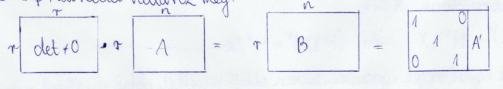
\includegraphics{matroid_ttest}
\centering
\end{figure}

\begin{theo} Grafikus matroidok tetszőleges test felett reprezentálhatók. \end{theo}
\begin{theo} Ha $M=(E,F)$ reprezentálható az $F$ test felett, akkor $M^{*}$ is. \end{theo}
\begin{theo} Ha $M=(E,F)$ reprezentálható az $F$ test felett, akkor minden minora is reprezentálható. \end{theo}
